\documentclass{article}
\usepackage{color}
\usepackage[utf8]{inputenc}
\usepackage{amsmath}
\usepackage{listings}
\usepackage{graphicx}
\usepackage{enumerate}

\title{CIS 419/519: Homework 4}
\author{\{Your name here\}}
\date{}

\begin{document}

\maketitle
    Although the solutions are my own, I consulted with the following people while working on this homework: \{Names here\} \\


\section*{Neural Networks}
\subsection*{Feed Forward}
Plots:
\begin{center}
    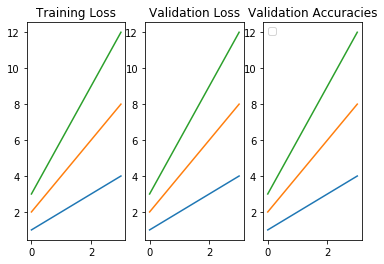
\includegraphics{example-plot.png} % Replace this image with your plot.
\end{center}

\begin{center}
    \begin{tabular}{|c|c|}
        \hline
        Learning Rate & Final Validation Accuracy \\
        \hline
        0.0001 & \\
        0.00005 & \\
        0.00001 & \\
        \hline
    \end{tabular}
\end{center}
Learning rate with best validation accuracy: XXX.
The test accuracy of that model is YYY.

\subsection*{Convolutional}
Plots:
\begin{center}
    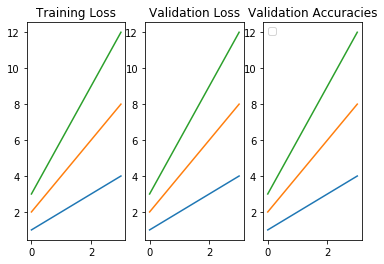
\includegraphics{example-plot.png} % Replace this image with your plot.
\end{center}

\begin{center}
    \begin{tabular}{|c|c|}
        \hline
        Learning Rate & Final Validation Accuracy \\
        \hline
        0.01 & \\
        0.001 & \\
        0.0001 & \\
        \hline
    \end{tabular}
\end{center}
Learning rate with best validation accuracy: XXX.
The test accuracy of that model is YYY.

\section*{Document Classification}

\begin{center}
    \begin{tabular}{|c|c|c|}
        \hline
        Representation & $k$ & Test Accuracy \\
        \hline
        BBoW & - & - \\
        CBoW & - & - \\
        TF-IDF & - & - \\
        \hline
    \end{tabular}
\end{center}

What impact does $k$ have?
That is, as the value of $k$ goes to infinity, what will happen to $P(y \mid d)$?


\section*{Theory}
\subsection*{Multivariate Exponential Naive Bayes}
\begin{enumerate}
    \item
        \begin{center}
            \begin{tabular}{|rp{1in}|rp{1in}|}
                \hline
                $P(Y\tight{=}A)=$ & & $P(Y\tight{=}B)=$ & \\ \hline
                $\lambda_{A;1}=$ & & $\lambda_{B;1}=$ & \\ \hline
                $\lambda_{A;2}=$ & & $\lambda_{B;2}=$ & \\ \hline
            \end{tabular}
        \end{center}
    \item
    \item
    \item
    \item
\end{enumerate}

\subsection*{Coin Toss}
The most likely value of $p$ is ... and here's why.

\end{document}
